% MATLAB source: paper/plot_existing_manuscript_figures.m
\begin{figure}[tbp]
  \centering
  \begin{subfigure}[t]{0.315\linewidth}
    \centering
    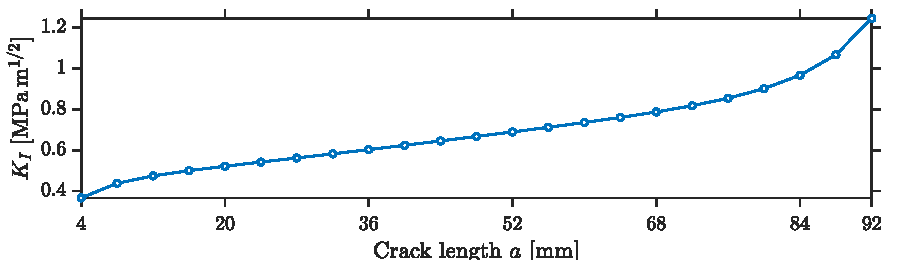
\includegraphics[width=\linewidth]{figures/intensities/KI.pdf}
    \caption{Opening-mode factor $K_I$.}
    \label{fig:intensities-KI}
  \end{subfigure}
  \hfill
  \begin{subfigure}[t]{0.315\linewidth}
    \centering
    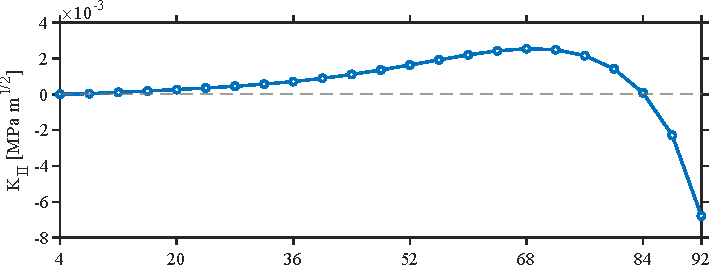
\includegraphics[width=\linewidth]{figures/intensities/KII.pdf}
    \caption{Sliding-mode factor $K_{II}$.}
    \label{fig:intensities-KII}
  \end{subfigure}
  \hfill
  \begin{subfigure}[t]{0.315\linewidth}
    \centering
    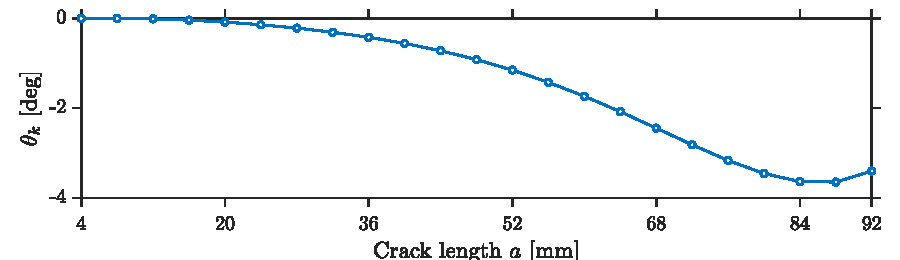
\includegraphics[width=\linewidth]{figures/intensities/theta.pdf}
    \caption{Absolute direction $\theta_k$.}
    \label{fig:intensities-theta}
  \end{subfigure}

  \caption{Accepted intensities and absolute direction in the frozen
  initiation frame. Intensities correspond to unit remote traction. The
  direction minimum occurs at $P_{22}$; positive turning there produces the
  less negative $P_{23}$ direction. No physical curve includes $P_{24}$.}
  \label{fig:intensities}
\end{figure}
